\section{setup}

\subsection{Individual components}
\paragraph{Drift chamber}
is a type of gaseous ionization detector. As its name suggest, it detects ionizing particles by a electric field inside. When the gas atoms get ionized, the electron will transport to the anode and generate a signal. Especially near the anode wire, the electric field is so huge that the electron becomes ionizing itself and cause further discharge. This effect is called avalanche~\cite{leo}. Obviously, number of ions collected at anode depends strongly on the voltage put between anode and cathode.

\begin{figure}[htpb]
	\centering
	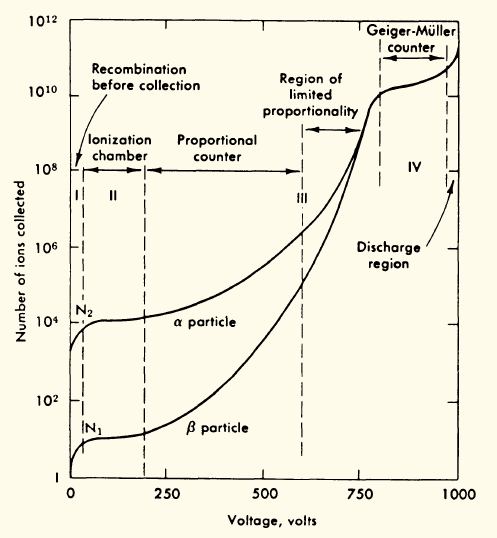
\includegraphics[width=0.5\linewidth]{voltage-diagram.png}
	\caption{Example diagram of number of ions versus applied voltage in a single wire gas chamber~\cite{leo}. Note that vertical axis is in logarithmic scale. }%
	\label{fig:voltage-diagram}
\end{figure}
An exemplar development of number of ions with increasing voltage is shown in figure~\ref{fig:voltage-diagram}. In this setup, we essentially want to saturate the gas chamber (thus to region IV in figure~\ref{fig:voltage-diagram}) so that it can reliably count the ionizing particles regardless of their energy.

In this experiment, there are three drift chamber modules. In each of these, there are three layers of $88$ straws~\cite{manual}.

\paragraph{Scintillator and PMT}
work as external trigger here. They together are able to convert ionizing particle into relatively low energy photons (scintillator), convert photon into electrons using photoelectric effect, and finally with electric field to multiply the number of electrons to generate visible signals~\cite{wermes}. Here two such detectors are used, one on top of the drift chamber and on below~\cite{manual}.

\paragraph{Shaper}
A shaper is a module which turns inputs pulse into logic signals of standard levels and fixed width~\cite{leo}.

\paragraph{TDC}
stands for Time-to-Digital Converter measures the time between two signals and gives the time difference of these two~\cite{leo}.

\paragraph{Coincidence unit}
determines if two or more logic signals overlap with each other within a preset time intervals and output signal if true and no signal if false. The present time is called resolving time. It can be implemented with a transmission gate or simply summing and passing through a discriminator~\cite{leo}.

\subsection{Whole setup}
\begin{figure}[ht]
	\centering
	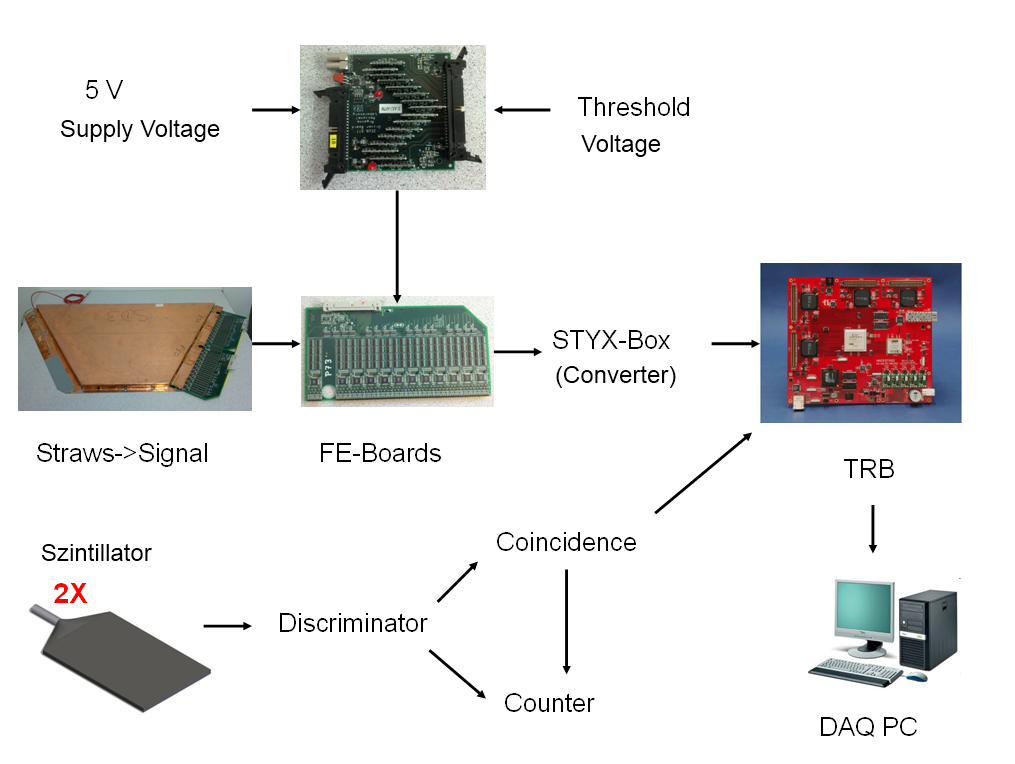
\includegraphics[width=0.6\linewidth]{setup-schematic.png}
	\caption{Schematics of the experiment setup~\cite{manual}.}%
	\label{fig:setup}
\end{figure}
Schematically the setup is like in figure~\ref{fig:setup}. The front end boards (FE-boards) are attached to the straws. The boards contain amplifiers, shapers and discriminators, so that as long as input signal pass a set threshold, a logic signal is generated. The threshold voltage can be set on an external power supply. As for the trigger part, the signal will need to pass discriminators (to filter out noises) and goes to a coincidence unit. The coincidence unit makes sure that an event is only recorded when it flies through both scintillators. In the end, signals from straw modules and scintillator units go into TRB board and to the PC~\cite{manual}.
